\section[MODELO DE ARQUITETURA]{MODELO DE ARQUITETURA}

O modelo de arquitetura no seu nível mais elevado, pode ser visto como um modelo de três camadas, conforme a figura \ref{camadas_arquitetura}.
\begin{figure}[ht]
	\centering
	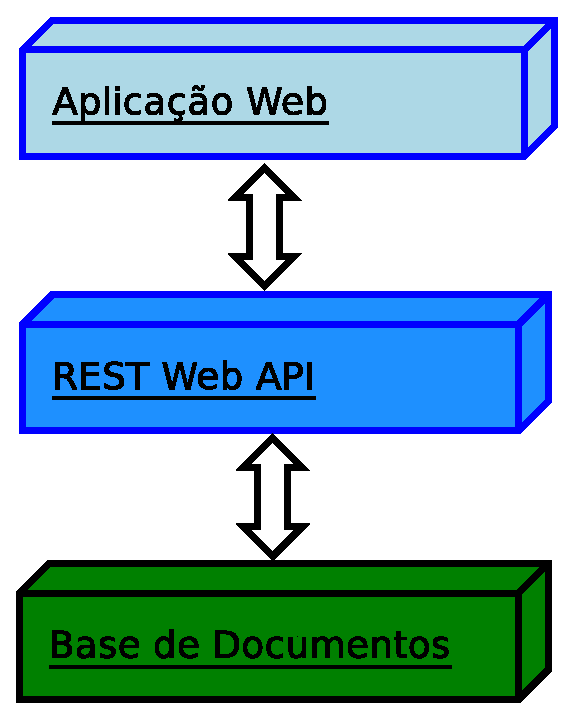
\includegraphics[width=7cm]{figuras/camadas.eps}
	\caption{Camadas arquiteturais}
	\label{camadas_arquitetura}
\end{figure}

A camada web é responsável pela interação com o usuário. 
A camada \emph{Web API} é responsável pela lógica de negócio. 
A camada de base de documentos é responsável pela persistência dos dados da aplicação.


\subsection[CAMADA DE APLICAÇÃO WEB] {CAMADA DE APLICAÇÃO WEB}
Esta camada foi projetada para rodar em \emph{browsers} que suportam HTML 5. 
Ela é desenvolvida usando-se Javascript, CSS e HTML. Além disso, adotou-se o \emph{framework} de desenvolvimento web \emph{AngularJS}. \cite{Branas2014} é um guia introdutório conciso no assunto. 
Segundo \cite{Freeman2014}, outro guia no assunto, o \emph{AngularJS} se baseia no padrão de projeto \emph{Model-View-Controller} (MVC), e sua enfase é em permitir a criação de aplicações: extensíveis, manuteníveis, testáveis e padronizadas.

Como, até o momento de conclusão deste trabalho, o projeto não conta com um \emph{web designer}, uma solução técnica para minimizar as consequências deste problema, teve de ser adotada. Os usuários finais do software, profissionais da área de saúde, dificilmente se interessariam pelo mesmo sem uma interface atraente e amigável.
A solução adotada foi utilizar a biblioteca \emph{angular-material}. 
Esta biblioteca, como indicado pelo seu nome, é construída com o \emph{AngularJS}. 
Ela disponibiliza serviços e diretivas que podem ser usados para construir a interface gráfica da aplicação. 
Diretivas são componentes que podem ser inseridos diretamente no código HTML da aplicação, dando a aparência de estender a própria HTML. 
Por exemplo a diretiva \emph{md-button} da biblioteca, é um tipo de botão que não é próprio do HTML. 
Outros exemplos de diretivas são: caixas de diálogos, barras de ferramentas, barras de progresso, grades, \emph{tooltip}, etc. 
Esta biblioteca é baseada na especificação \emph{Material Design} criada pela empresa Google. 
A especificação discorre sobre padrões de designe gráfico e interação com usuário e é baseada no princípio da metáfora de materiais. 
Esta metáfora é uma teoria unificada de um espaço racionalizado e sistemas de movimento, isto segundo \cite{Google2015a}. Outra vantagem da biblioteca é que ela é projetada para se adaptar a diferentes tipos de dispositivos com telas de tamanhos diferentes.
